\documentclass{article}
\usepackage[margin=1in]{geometry}
\usepackage{amsmath,amsthm,amssymb}
\usepackage{bbm,enumerate,mathtools}
\usepackage{tikz,pgfplots}
\usepackage{chessboard}
\usepackage[hidelinks]{hyperref}
\usepackage{multicol} % Problem 35

\newenvironment{question}{\begin{trivlist}\item[\textbf{Question.}]}{\end{trivlist}}
\newenvironment{note}{\begin{trivlist}\item[\textbf{Note.}]}{\end{trivlist}}
\newenvironment{references}{\begin{trivlist}\item[\textbf{References.}]}{\end{trivlist}}
\newenvironment{related}{\begin{trivlist}\item[\textbf{Related.}]\end{trivlist}\begin{enumerate}}{\end{enumerate}}


\begin{document}
\rating{2}{1}
Starting with $1$ and working in a hexagonal spiral, repeatedly choose the
smallest positive integer such that it won't be adjacent either itself (once)
or to the same number twice.
\begin{figure}[!h]
  \centering
  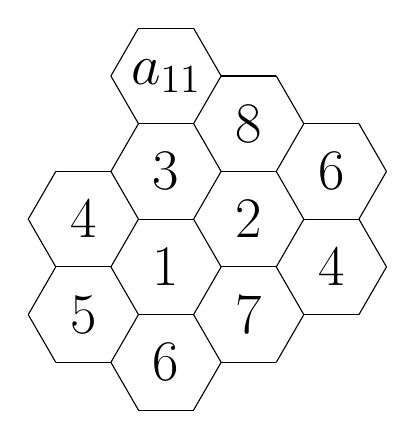
\begin{tikzpicture}[scale=0.7]

    \foreach \x in {0} {
      \foreach \y in {0} {
        \node at (\x, \y) {\huge 1};
        \draw (\x-1,\y)--(\x-0.5,{\y + sqrt(3)/2});
        \draw (\x-0.5,{\y + sqrt(3)/2})--(\x+0.5,{\y + sqrt(3)/2});
        \draw (\x+0.5,{\y + sqrt(3)/2})--(\x+1,\y);
        \draw (\x+1,\y)--(\x+0.5,{\y - sqrt(3)/2});
        \draw (\x+0.5,{\y - sqrt(3)/2})--(\x-0.5,{\y - sqrt(3)/2});
        \draw (\x-0.5,{\y - sqrt(3)/2})--(\x-1,\y);
      }
    }

    \foreach \x in {1.5} {
      \foreach \y in {0.8660254038} {
        \node at (\x, \y) {\huge 2};
        \draw (\x-1,\y)--(\x-0.5,{\y + sqrt(3)/2});
        \draw (\x-0.5,{\y + sqrt(3)/2})--(\x+0.5,{\y + sqrt(3)/2});
        \draw (\x+0.5,{\y + sqrt(3)/2})--(\x+1,\y);
        \draw (\x+1,\y)--(\x+0.5,{\y - sqrt(3)/2});
        \draw (\x+0.5,{\y - sqrt(3)/2})--(\x-0.5,{\y - sqrt(3)/2});
      }
    }

    \foreach \x in {0} {
      \foreach \y in {2 * 0.8660254038} {
        \node at (\x, \y) {\huge 3};
        \draw (\x-1,\y)--(\x-0.5,{\y + sqrt(3)/2});
        \draw (\x-0.5,{\y + sqrt(3)/2})--(\x+0.5,{\y + sqrt(3)/2});
        \draw (\x+0.5,{\y + sqrt(3)/2})--(\x+1,\y);
        \draw (\x-0.5,{\y - sqrt(3)/2})--(\x-1,\y);
      }
    }

    \foreach \x in {-1.5} {
      \foreach \y in {0.8660254038} {
        \node at (\x, \y) {\huge 4};
        \draw (\x-1,\y)--(\x-0.5,{\y + sqrt(3)/2});
        \draw (\x-0.5,{\y + sqrt(3)/2})--(\x+0.5,{\y + sqrt(3)/2});
        \draw (\x+0.5,{\y - sqrt(3)/2})--(\x-0.5,{\y - sqrt(3)/2});
        \draw (\x-0.5,{\y - sqrt(3)/2})--(\x-1,\y);
      }
    }

    \foreach \x in {-1.5} {
      \foreach \y in {-0.8660254038} {
        \node at (\x, \y) {\huge 5};
        \draw (\x-1,\y)--(\x-0.5,{\y + sqrt(3)/2});
        \draw (\x+1,\y)--(\x+0.5,{\y - sqrt(3)/2});
        \draw (\x+0.5,{\y - sqrt(3)/2})--(\x-0.5,{\y - sqrt(3)/2});
        \draw (\x-0.5,{\y - sqrt(3)/2})--(\x-1,\y);
      }
    }

    \foreach \x in {0} {
      \foreach \y in {-2 * 0.8660254038} {
        \node at (\x, \y) {\huge 6};
        \draw (\x+0.5,{\y + sqrt(3)/2})--(\x+1,\y);
        \draw (\x+1,\y)--(\x+0.5,{\y - sqrt(3)/2});
        \draw (\x+0.5,{\y - sqrt(3)/2})--(\x-0.5,{\y - sqrt(3)/2});
        \draw (\x-0.5,{\y - sqrt(3)/2})--(\x-1,\y);
      }
    }

    \foreach \x in {1.5} {
      \foreach \y in {-0.8660254038} {
        \node at (\x, \y) {\huge 7};
        \draw (\x+0.5,{\y + sqrt(3)/2})--(\x+1,\y);
        \draw (\x+1,\y)--(\x+0.5,{\y - sqrt(3)/2});
        \draw (\x+0.5,{\y - sqrt(3)/2})--(\x-0.5,{\y - sqrt(3)/2});
      }
    }

    \foreach \x in {3} {
      \foreach \y in {0} {
        \node at (\x, \y) {\huge 4};
        \draw (\x-0.5,{\y + sqrt(3)/2})--(\x+0.5,{\y + sqrt(3)/2});
        \draw (\x+0.5,{\y + sqrt(3)/2})--(\x+1,\y);
        \draw (\x+1,\y)--(\x+0.5,{\y - sqrt(3)/2});
        \draw (\x+0.5,{\y - sqrt(3)/2})--(\x-0.5,{\y - sqrt(3)/2});
      }
    }

    \foreach \x in {3} {
      \foreach \y in {2 * 0.8660254038} {
        \node at (\x, \y) {\huge 6};
        \draw (\x-1,\y)--(\x-0.5,{\y + sqrt(3)/2});
        \draw (\x-0.5,{\y + sqrt(3)/2})--(\x+0.5,{\y + sqrt(3)/2});
        \draw (\x+0.5,{\y + sqrt(3)/2})--(\x+1,\y);
        \draw (\x+1,\y)--(\x+0.5,{\y - sqrt(3)/2});
      }
    }

    \foreach \x in {1.5} {
      \foreach \y in {3*0.8660254038} {
        \node at (\x, \y) {\huge 8};
        \draw (\x-1,\y)--(\x-0.5,{\y + sqrt(3)/2});
        \draw (\x-0.5,{\y + sqrt(3)/2})--(\x+0.5,{\y + sqrt(3)/2});
        \draw (\x+0.5,{\y + sqrt(3)/2})--(\x+1,\y);
      }
    }

    \foreach \x in {0} {
      \foreach \y in {4 * 0.8660254038} {
        \node at (\x, \y) {\huge $a_{11}$};
        \draw (\x-1,\y)--(\x-0.5,{\y + sqrt(3)/2});
        \draw (\x-0.5,{\y + sqrt(3)/2})--(\x+0.5,{\y + sqrt(3)/2});
        \draw (\x+0.5,{\y + sqrt(3)/2})--(\x+1,\y);
        \draw (\x-0.5,{\y - sqrt(3)/2})--(\x-1,\y);
      }
    }
  \end{tikzpicture}\hspace{1cm}
  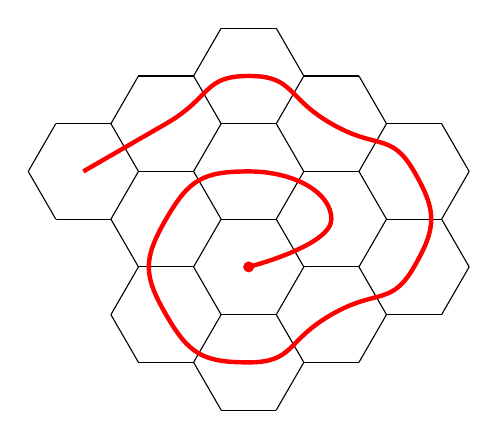
\begin{tikzpicture}[scale=0.7]

    \foreach \x in {0} {
      \foreach \y in {0} {
        \draw (\x-1,\y)--(\x-0.5,{\y + sqrt(3)/2});
        \draw (\x-0.5,{\y + sqrt(3)/2})--(\x+0.5,{\y + sqrt(3)/2});
        \draw (\x+0.5,{\y + sqrt(3)/2})--(\x+1,\y);
        \draw (\x+1,\y)--(\x+0.5,{\y - sqrt(3)/2});
        \draw (\x+0.5,{\y - sqrt(3)/2})--(\x-0.5,{\y - sqrt(3)/2});
        \draw (\x-0.5,{\y - sqrt(3)/2})--(\x-1,\y);
      }
    }
    \foreach \x in {1.5} {
      \foreach \y in {0.8660254038} {
        \draw (\x-1,\y)--(\x-0.5,{\y + sqrt(3)/2});
        \draw (\x-0.5,{\y + sqrt(3)/2})--(\x+0.5,{\y + sqrt(3)/2});
        \draw (\x+0.5,{\y + sqrt(3)/2})--(\x+1,\y);
        \draw (\x+1,\y)--(\x+0.5,{\y - sqrt(3)/2});
        \draw (\x+0.5,{\y - sqrt(3)/2})--(\x-0.5,{\y - sqrt(3)/2});
      }
    }
    \foreach \x in {0} {
      \foreach \y in {2 * 0.8660254038} {
        \draw (\x-1,\y)--(\x-0.5,{\y + sqrt(3)/2});
        \draw (\x-0.5,{\y + sqrt(3)/2})--(\x+0.5,{\y + sqrt(3)/2});
        \draw (\x+0.5,{\y + sqrt(3)/2})--(\x+1,\y);
        \draw (\x-0.5,{\y - sqrt(3)/2})--(\x-1,\y);
      }
    }
    \foreach \x in {-1.5} {
      \foreach \y in {0.8660254038} {
        \draw (\x-1,\y)--(\x-0.5,{\y + sqrt(3)/2});
        \draw (\x-0.5,{\y + sqrt(3)/2})--(\x+0.5,{\y + sqrt(3)/2});
        \draw (\x+0.5,{\y - sqrt(3)/2})--(\x-0.5,{\y - sqrt(3)/2});
        \draw (\x-0.5,{\y - sqrt(3)/2})--(\x-1,\y);
      }
    }

    \foreach \x in {-1.5} {
      \foreach \y in {-0.8660254038} {
        \draw (\x-1,\y)--(\x-0.5,{\y + sqrt(3)/2});
        \draw (\x+1,\y)--(\x+0.5,{\y - sqrt(3)/2});
        \draw (\x+0.5,{\y - sqrt(3)/2})--(\x-0.5,{\y - sqrt(3)/2});
        \draw (\x-0.5,{\y - sqrt(3)/2})--(\x-1,\y);
      }
    }

    \foreach \x in {0} {
      \foreach \y in {-2 * 0.8660254038} {
        \draw (\x+0.5,{\y + sqrt(3)/2})--(\x+1,\y);
        \draw (\x+1,\y)--(\x+0.5,{\y - sqrt(3)/2});
        \draw (\x+0.5,{\y - sqrt(3)/2})--(\x-0.5,{\y - sqrt(3)/2});
        \draw (\x-0.5,{\y - sqrt(3)/2})--(\x-1,\y);
      }
    }

    \foreach \x in {1.5} {
      \foreach \y in {-0.8660254038} {
        \draw (\x+0.5,{\y + sqrt(3)/2})--(\x+1,\y);
        \draw (\x+1,\y)--(\x+0.5,{\y - sqrt(3)/2});
        \draw (\x+0.5,{\y - sqrt(3)/2})--(\x-0.5,{\y - sqrt(3)/2});
      }
    }

    \foreach \x in {3} {
      \foreach \y in {0} {
        \draw (\x-0.5,{\y + sqrt(3)/2})--(\x+0.5,{\y + sqrt(3)/2});
        \draw (\x+0.5,{\y + sqrt(3)/2})--(\x+1,\y);
        \draw (\x+1,\y)--(\x+0.5,{\y - sqrt(3)/2});
        \draw (\x+0.5,{\y - sqrt(3)/2})--(\x-0.5,{\y - sqrt(3)/2});
      }
    }

    \foreach \x in {3} {
      \foreach \y in {2 * 0.8660254038} {
        \draw (\x-1,\y)--(\x-0.5,{\y + sqrt(3)/2});
        \draw (\x-0.5,{\y + sqrt(3)/2})--(\x+0.5,{\y + sqrt(3)/2});
        \draw (\x+0.5,{\y + sqrt(3)/2})--(\x+1,\y);
        \draw (\x+1,\y)--(\x+0.5,{\y - sqrt(3)/2});
      }
    }

    \foreach \x in {1.5} {
      \foreach \y in {3*0.8660254038} {
        \draw (\x-1,\y)--(\x-0.5,{\y + sqrt(3)/2});
        \draw (\x-0.5,{\y + sqrt(3)/2})--(\x+0.5,{\y + sqrt(3)/2});
        \draw (\x+0.5,{\y + sqrt(3)/2})--(\x+1,\y);
      }
    }

    \foreach \x in {0} {
      \foreach \y in {4 * 0.8660254038} {
        \draw (\x-1,\y)--(\x-0.5,{\y + sqrt(3)/2});
        \draw (\x-0.5,{\y + sqrt(3)/2})--(\x+0.5,{\y + sqrt(3)/2});
        \draw (\x+0.5,{\y + sqrt(3)/2})--(\x+1,\y);
        \draw (\x-0.5,{\y - sqrt(3)/2})--(\x-1,\y);
      }
    }

    \foreach \x in {-1.5} {
      \foreach \y in {3*0.8660254038} {
        \draw (\x-1,\y)--(\x-0.5,{\y + sqrt(3)/2});
        \draw (\x-0.5,{\y + sqrt(3)/2})--(\x+0.5,{\y + sqrt(3)/2});
        \draw (\x-0.5,{\y - sqrt(3)/2})--(\x-1,\y);
      }
    }

    \foreach \x in {-3} {
      \foreach \y in {2*0.8660254038} {
        \draw (\x-1,\y)--(\x-0.5,{\y + sqrt(3)/2});
        \draw (\x-0.5,{\y + sqrt(3)/2})--(\x+0.5,{\y + sqrt(3)/2});
        \draw (\x+0.5,{\y - sqrt(3)/2})--(\x-0.5,{\y - sqrt(3)/2});
        \draw (\x-0.5,{\y - sqrt(3)/2})--(\x-1,\y);
      }
    }

    \fill[red] (0,0) circle (0.1cm);
    \draw[red, ultra thick] plot [smooth,tension=1] coordinates {
      (0,0) (1.5,0.866) (0,2 * 0.8660254038) (-1.5,0.866) (-1.5,-0.866)
      (0,-2*0.866) (1.5,-0.866) (3,0) (3, 2 * 0.8660254038)
      (1.5, 3*0.8660254038) (0, 4 * 0.8660254038) (-1.5, 3*0.8660254038)
      (-3, 2 * 0.8660254038)
    };

  \end{tikzpicture}
  \caption{
    $a_{11} \not= 1$ because $3$ is already adjacent to $1$,
    $a_{11} \not= 2$ because $3$ and $8$ are already adjacent to $2$,
    $a_{11} \not= 3$ because then $a_{11}$ would be equal to its neighbor,
    $a_{11} \not= 4$ because $3$ is already adjacent to $4$, thus
    $a_{11} = 5$.
  }
\end{figure}
\begin{figure}[!h]
  \centering
  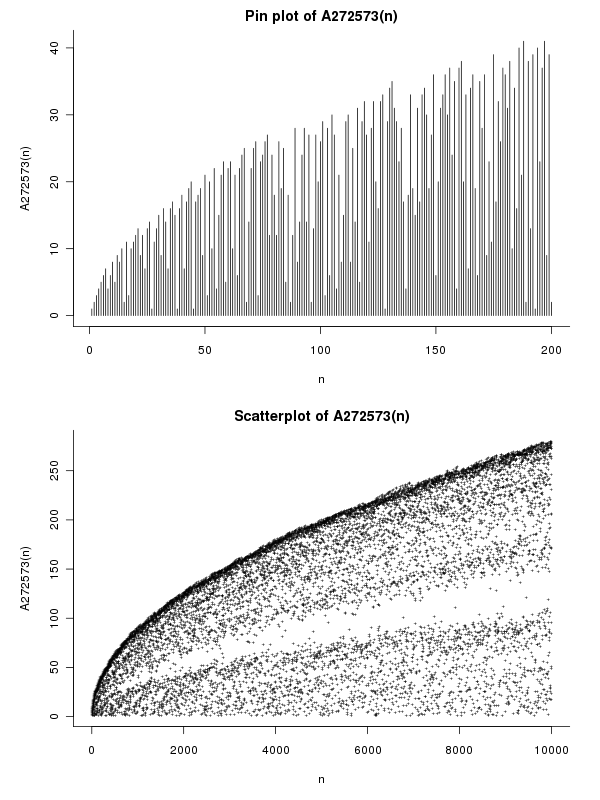
\includegraphics[trim={0 1.5cm 0 14cm},clip,scale=0.6]{assets/019_problem_A272573}
  \caption{A plot of $a_1$ through $a_{10000}$.}
\end{figure}


\begin{question}
  Why does a gap appear in the plot of the sequence?
\end{question}
\begin{references}
  \item \url{https://oeis.org/A272573}
\end{references}
\end{document}
